% !TEX root = ../main.tex
% Chapter 1

\chapter{Introduction}

\label{Chapter1} % For referencing the chapter elsewhere, use~\ref{Chapter1}

\lhead{Chapter 1. \emph{Introduction}} % This is for the header on each page - perhaps a shortened title

%----------------------------------------------------------------------------------------

\section{Outline}
\emph{Not intented for the reader.}
\begin{itemize}
  \item Context of research (\gls{har}), real-world applications
  \item Current methods, wrapper vs. filter methods
  \item Problem statement with current filter methods (which follows from \Cref{Chapter3} which goes in-depth with methods).
  \item Purpose of this research. E.g. "Find a better algorithm for short-activity segmentation"
  \item Provide the \emph{motivation} for this approach
  \item Relate to real-world applications
  \item Outline for rest of the thesis
\end{itemize}

-- Overall todo's --
\begin{itemize}
  \item \TODO{The term \emph{emperical data/distruction} is nowhere used in the thesis. or: Emperical cumulative distribution. Especially Chapter 2.}
  \item \TODO{Check for ``tang-constructions'': saying to much in a single sentence.}
  \item \TODO{Overall: meer focus op de \emph{waarom} vraag/antwoord bij keuzes. Bouwt aan motivatie en context van het geheel.}
  \item \TODO{Nu staat nog veel (met name Chapter 2) in ``aantekening'' style; ombouwen naar uitleggen, lezer begeleiden, duiden, verlaren etc.}
  \item \TODO{Test moet condenser: bepalen wat er uit gelaten mag worden.}
\end{itemize}

\begin{figure}
  \centering
    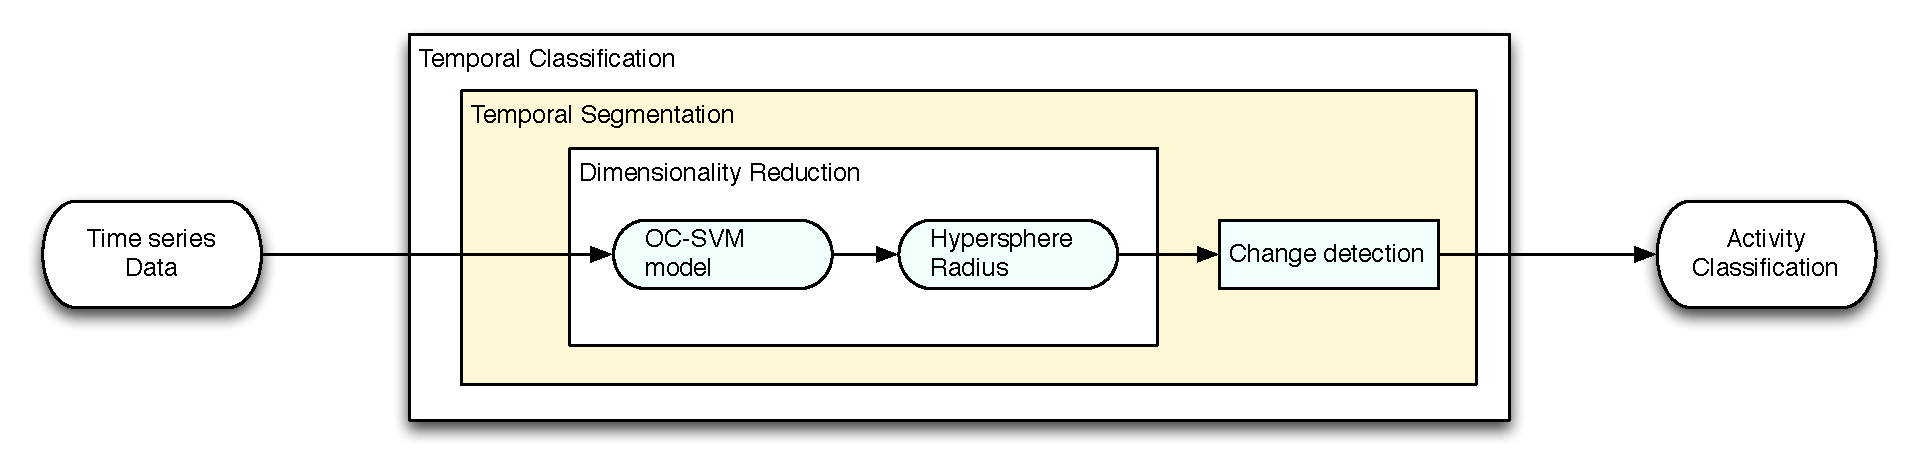
\includegraphics[width=\textwidth,height=\textheight,keepaspectratio]{./Figures/chapter1/thesis_goal.pdf}
  \caption[Thesis goal]{The goal of this thesis. The scope of this thesis is Temporal Segmentation, which can be useful in the context of Temporal Classification. Given a data set, we apply the construction of \gls{oc-svm} models as a form of dimensionality reduction. Using the reduced representation, being the radius $R$ of the constructed hypersphere, we apply direct change detection methods. The detected change points can support the classification of homogeneous segments of data.}
  \label{fig:thesis_goal}
\end{figure}


\begin{itemize}
  \item Begin with hook, statement, to draw attention
  \item Cite previous work and explain why new research was necessary.
  \item Statement of the goal of the thesis: why?
  \item Context to understand background of goal and the significance
  \item Acknowledgement of previous research and context
  \item Explain scope: what will be, and wont be discussed
  \item Verbal table of contents
  \item
\end{itemize}

Introduction to the introduction \\
Context \\
Restatement of problem and significance (echo of opening, but now with the context) \\
Restatement of the response \\
Roadmap \\

\section{Intro to intro}
With the wide availability of smartphones and built-in inertial sensors, more and more applications of \gls{har} are introduced.
Many approaches to recognizing the performed activity rely on classification of recorded data, which can be done online or in batches after the performance.
Often an time-windowed based approach is used, which feeds short consecutive segments of data through a model construction phase.
The constructed model is used to determine what (earlier learned) activity is performed.
Besides the explicit classification of the data, an implicit result is a segmentation of performed activities over time.

In this thesis the goal is to find the temporal segmentation of time series data explicitly, prior to the classification of the activities.
This is done under the assumption that it could be beneficial for classification methods to possess this explicit segmentation, since the model construction phase can use more data than the time-windowed approach would allow.
To find the temporal segmentation, we rely on change detection in time series data.
In the context of this research, this time series data consist of recordings from inertial sensors found in smartphones, during the performance of human activities.
We have recorded both in- and outdoor activities in an uncontrolled environment and in a continuous manner.

For the change detection algorithm we have used a special form of \gls{svm}, the \gls{oc-svm} based \gls{svdd} as introduced by Tax~\cite{tax2001one}.
This method models the data under consideration in the shape of a high-dimensional hypersphere.
From this hypersphere the radius is extracted, since a change in data characteristics (resulting from a change in performed activity) should result in a change of radius.





\section{Thesis structure}
The structure of this thesis is as follows.
In \Cref{Chapter2} a literature review is provided.
We will look at the different interpretations and implementations for change, novelty, and outlier detection.
Previous work in the field of \gls{har} is discussed and we end with existing applications of \glspl{svm} to change detection.
The next chapter further analyses \glspl{svm} and two implementations of \glspl{oc-svm}.
It relates the properties of the constructed \gls{oc-svm} models to change detection in time series data.
That relation is applied to our problem formulation in \Cref{Chapter4}, where we construct our change detection method, based on the work of Camci~\cite{camci2010change}.
The two following chapters apply the method to both artificial and real-world data.
\Cref{Chapter5} show the objective performance of the method to artificial constructed data.
In \Cref{Chapter6} we apply the method to our self-recorded real-world data.
We show the ability of detecting change in \gls{har} data, recorded by inertial sensors.
This thesis is conclused in \Cref{Chapter7}, in which we reflect on the performed research and state possibilities for feature research.